% for landscape posters, use "a4paper, landscape"
\documentclass[a4paper]{article}
\usepackage{better_poster}
\usepackage{twemojis}
\usepackage{graphicx}
\usepackage{utfsym}
\usepackage{boisik}
\usepackage{fontawesome5}

% ---- fill in from here
% poster size - this will scale the poster to the given size.
% for landscape posters add ", landscape" to the postersize command.
\postersize{a0paper}

% authors
\title{Your wrists are crying out for zero-friction support that moves when they move.}
\author{by Dan "Crime Fog" Rust and Bruce Olson}

% type of poster: [exp]erimental results, [methods], [theory]
% Disclaimer: the original classification had "study" and "intervention" as separate categories. I group them under experimental results.
\newcommand\postertype{exp} % [exp],[methods],[theory]

\begin{document}
	
	% main point of your study
	\makefinding{
		Your wrists, \textbf{floating} in \textbf{luxurious} comfort. That's what \textbf{Chair Forces} brings to the table.}
	}
	
	
	% \makemain{
		% }{
		
		% }
	
	
	% the main text of your poster goes here
	\makemain{
		% you can have 1 or 2 columns
		\raggedcolumns
		\begin{multicols}{2}
			\section{\underline{Our WHY}}
			\begin{compactitem}
            	\item Dan had significant wrist pain from the angles and friction demanded by the office. \usym{270d}
				\item It was $\boisik{\nVDash}$ distracting. 
				\item He found some products that \emph{*could*} work well. 
				\item He had some strong magnets.
				\item \usym{1f59b} ...and the most comfortable product was born. \usym{1f59a}
			\end{compactitem}
			
	        \section{\underline{Methods}}
			\begin{compactitem}
         	   \item Wrist-rests {\scriptsize $+ $} swivel-magnets {\scriptsize $+ $} squishy cushion \textbf{\emph{= heaven}}.
				\item Veteran-owned. \twemoji{flag: United States}
				\item Assembled with \scalebox{1.5}{\twemoji{sparkling heart}} in the USA. 
			\end{compactitem}
			
			% this determines where your columns will be separated
			\columnbreak
			
			\section{\underline{Results} \fontawesome{\faMouse}}
			\includegraphics[width=\linewidth]{cartoon.png}
			
		\end{multicols}
	}
	% If you have extra figures or data to show
	\makeextracolumn{
		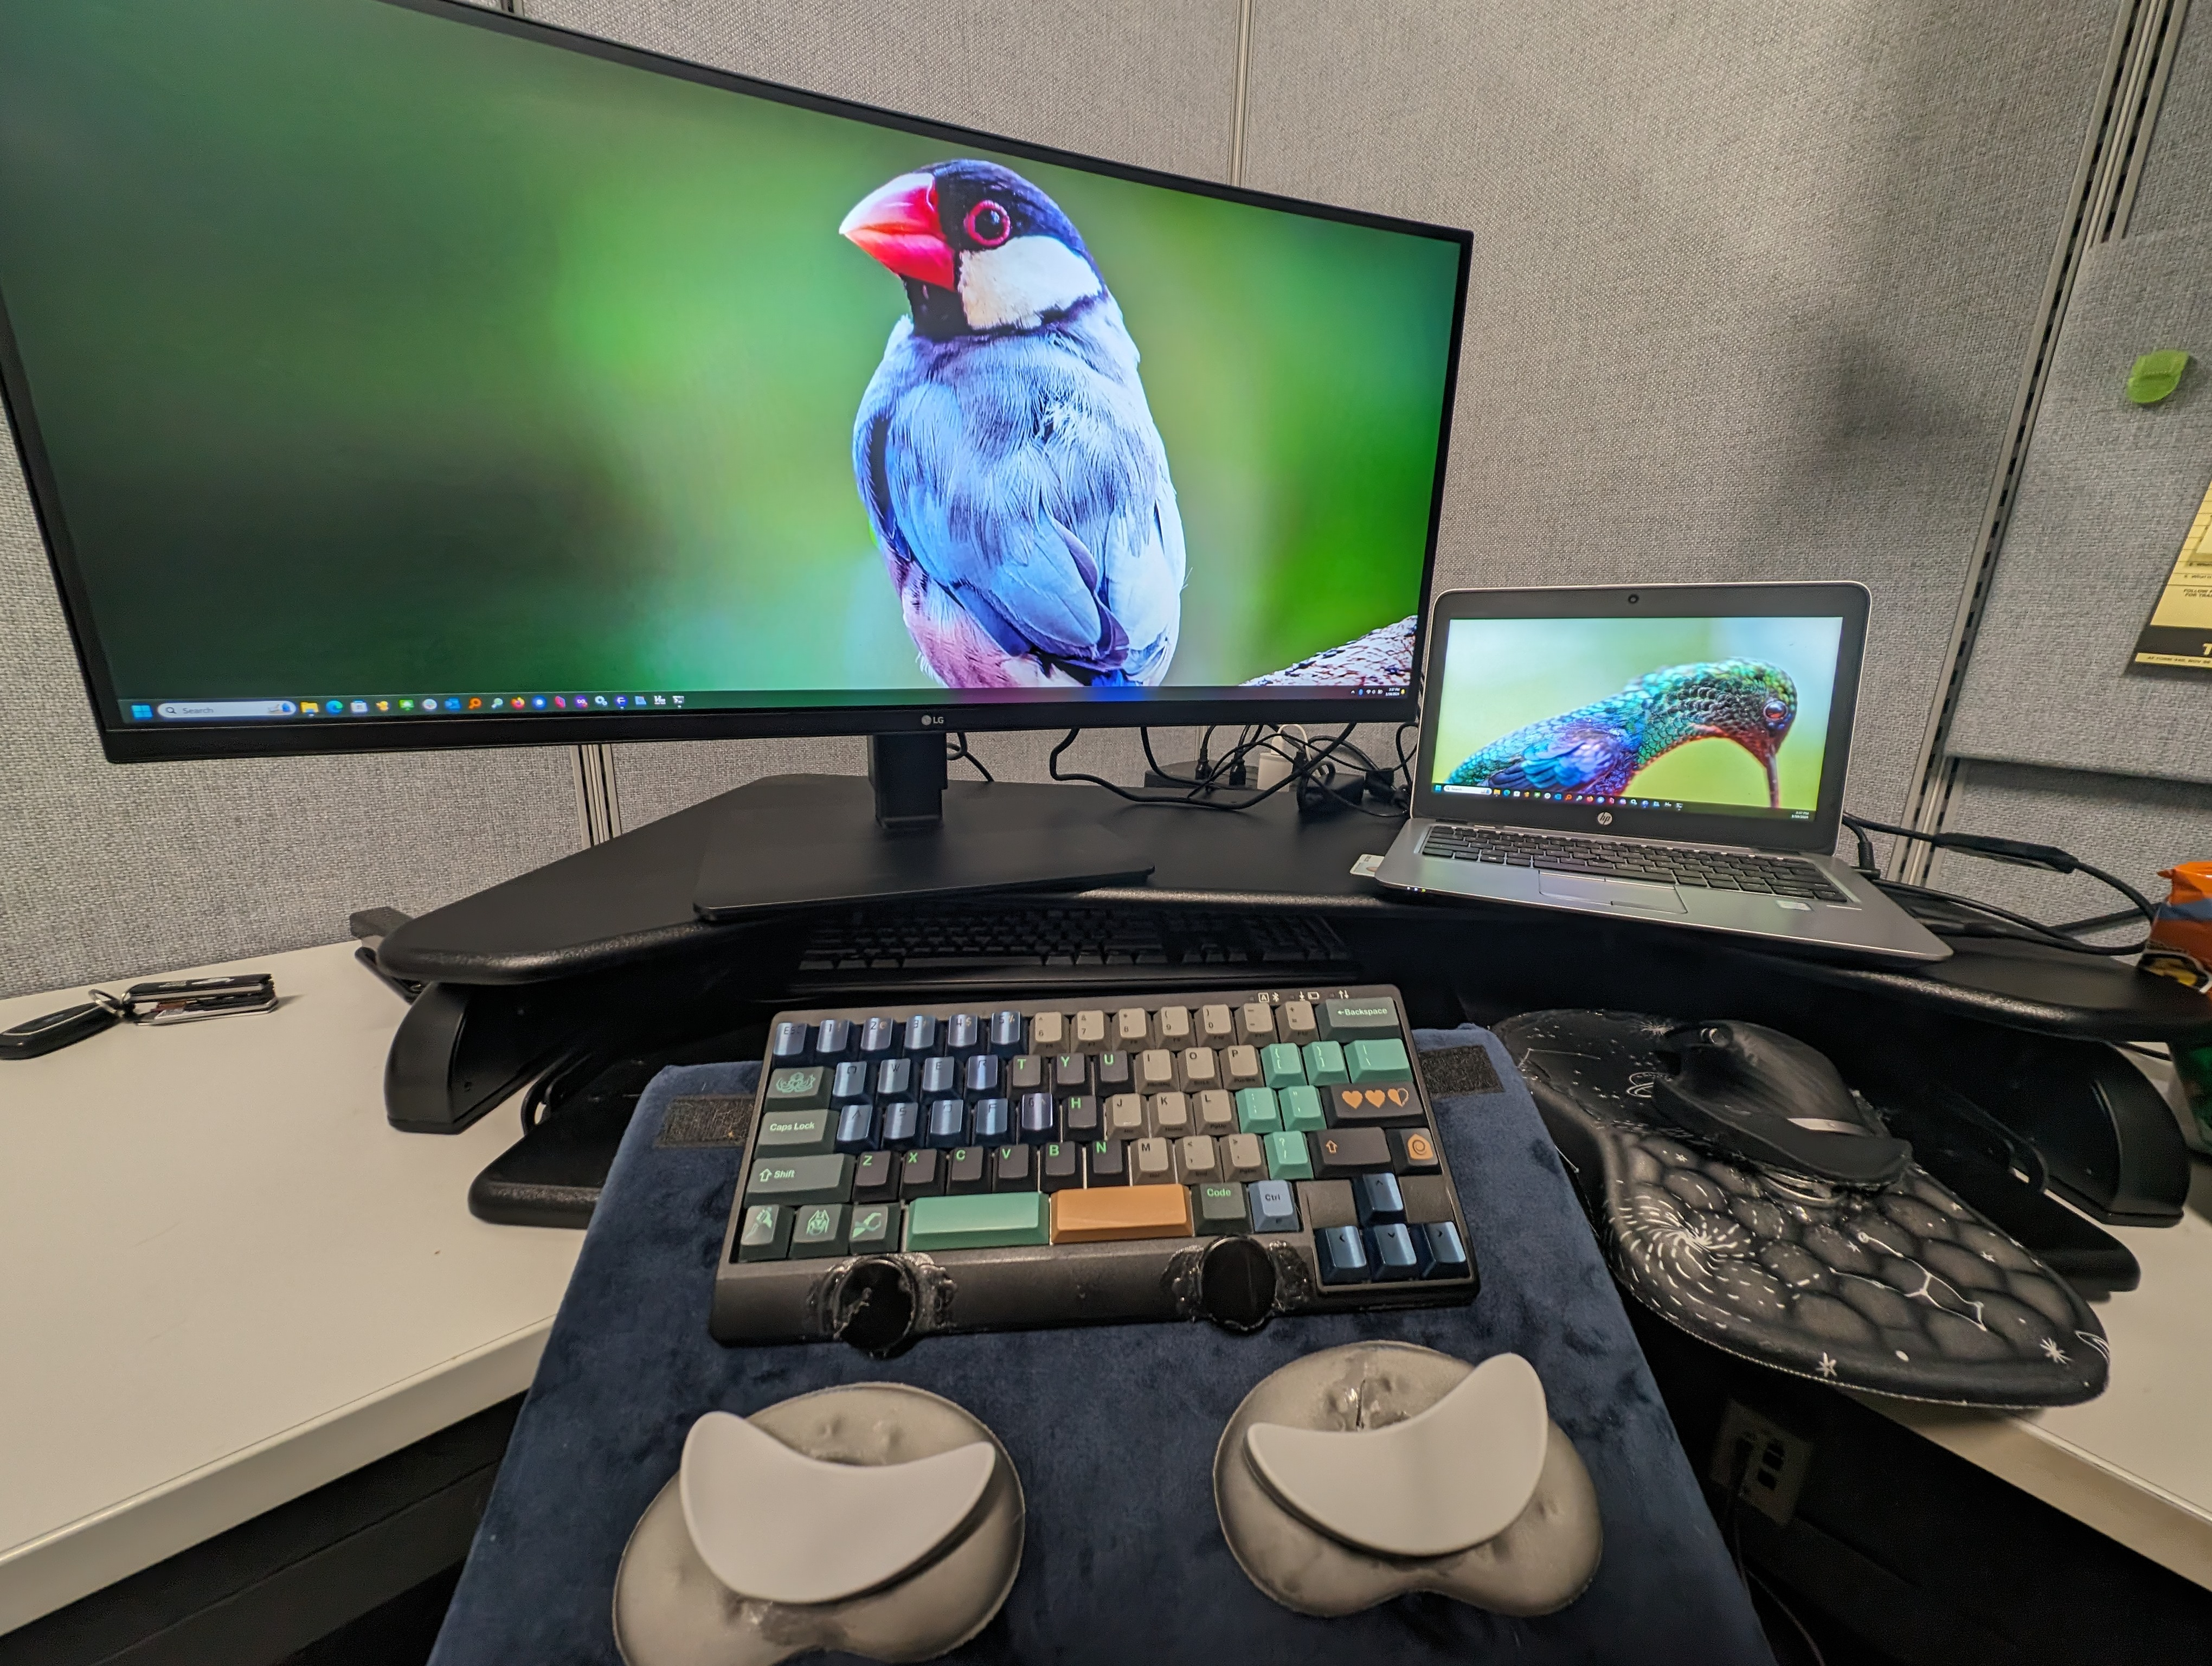
\includegraphics[width=\linewidth]{birds.png}
		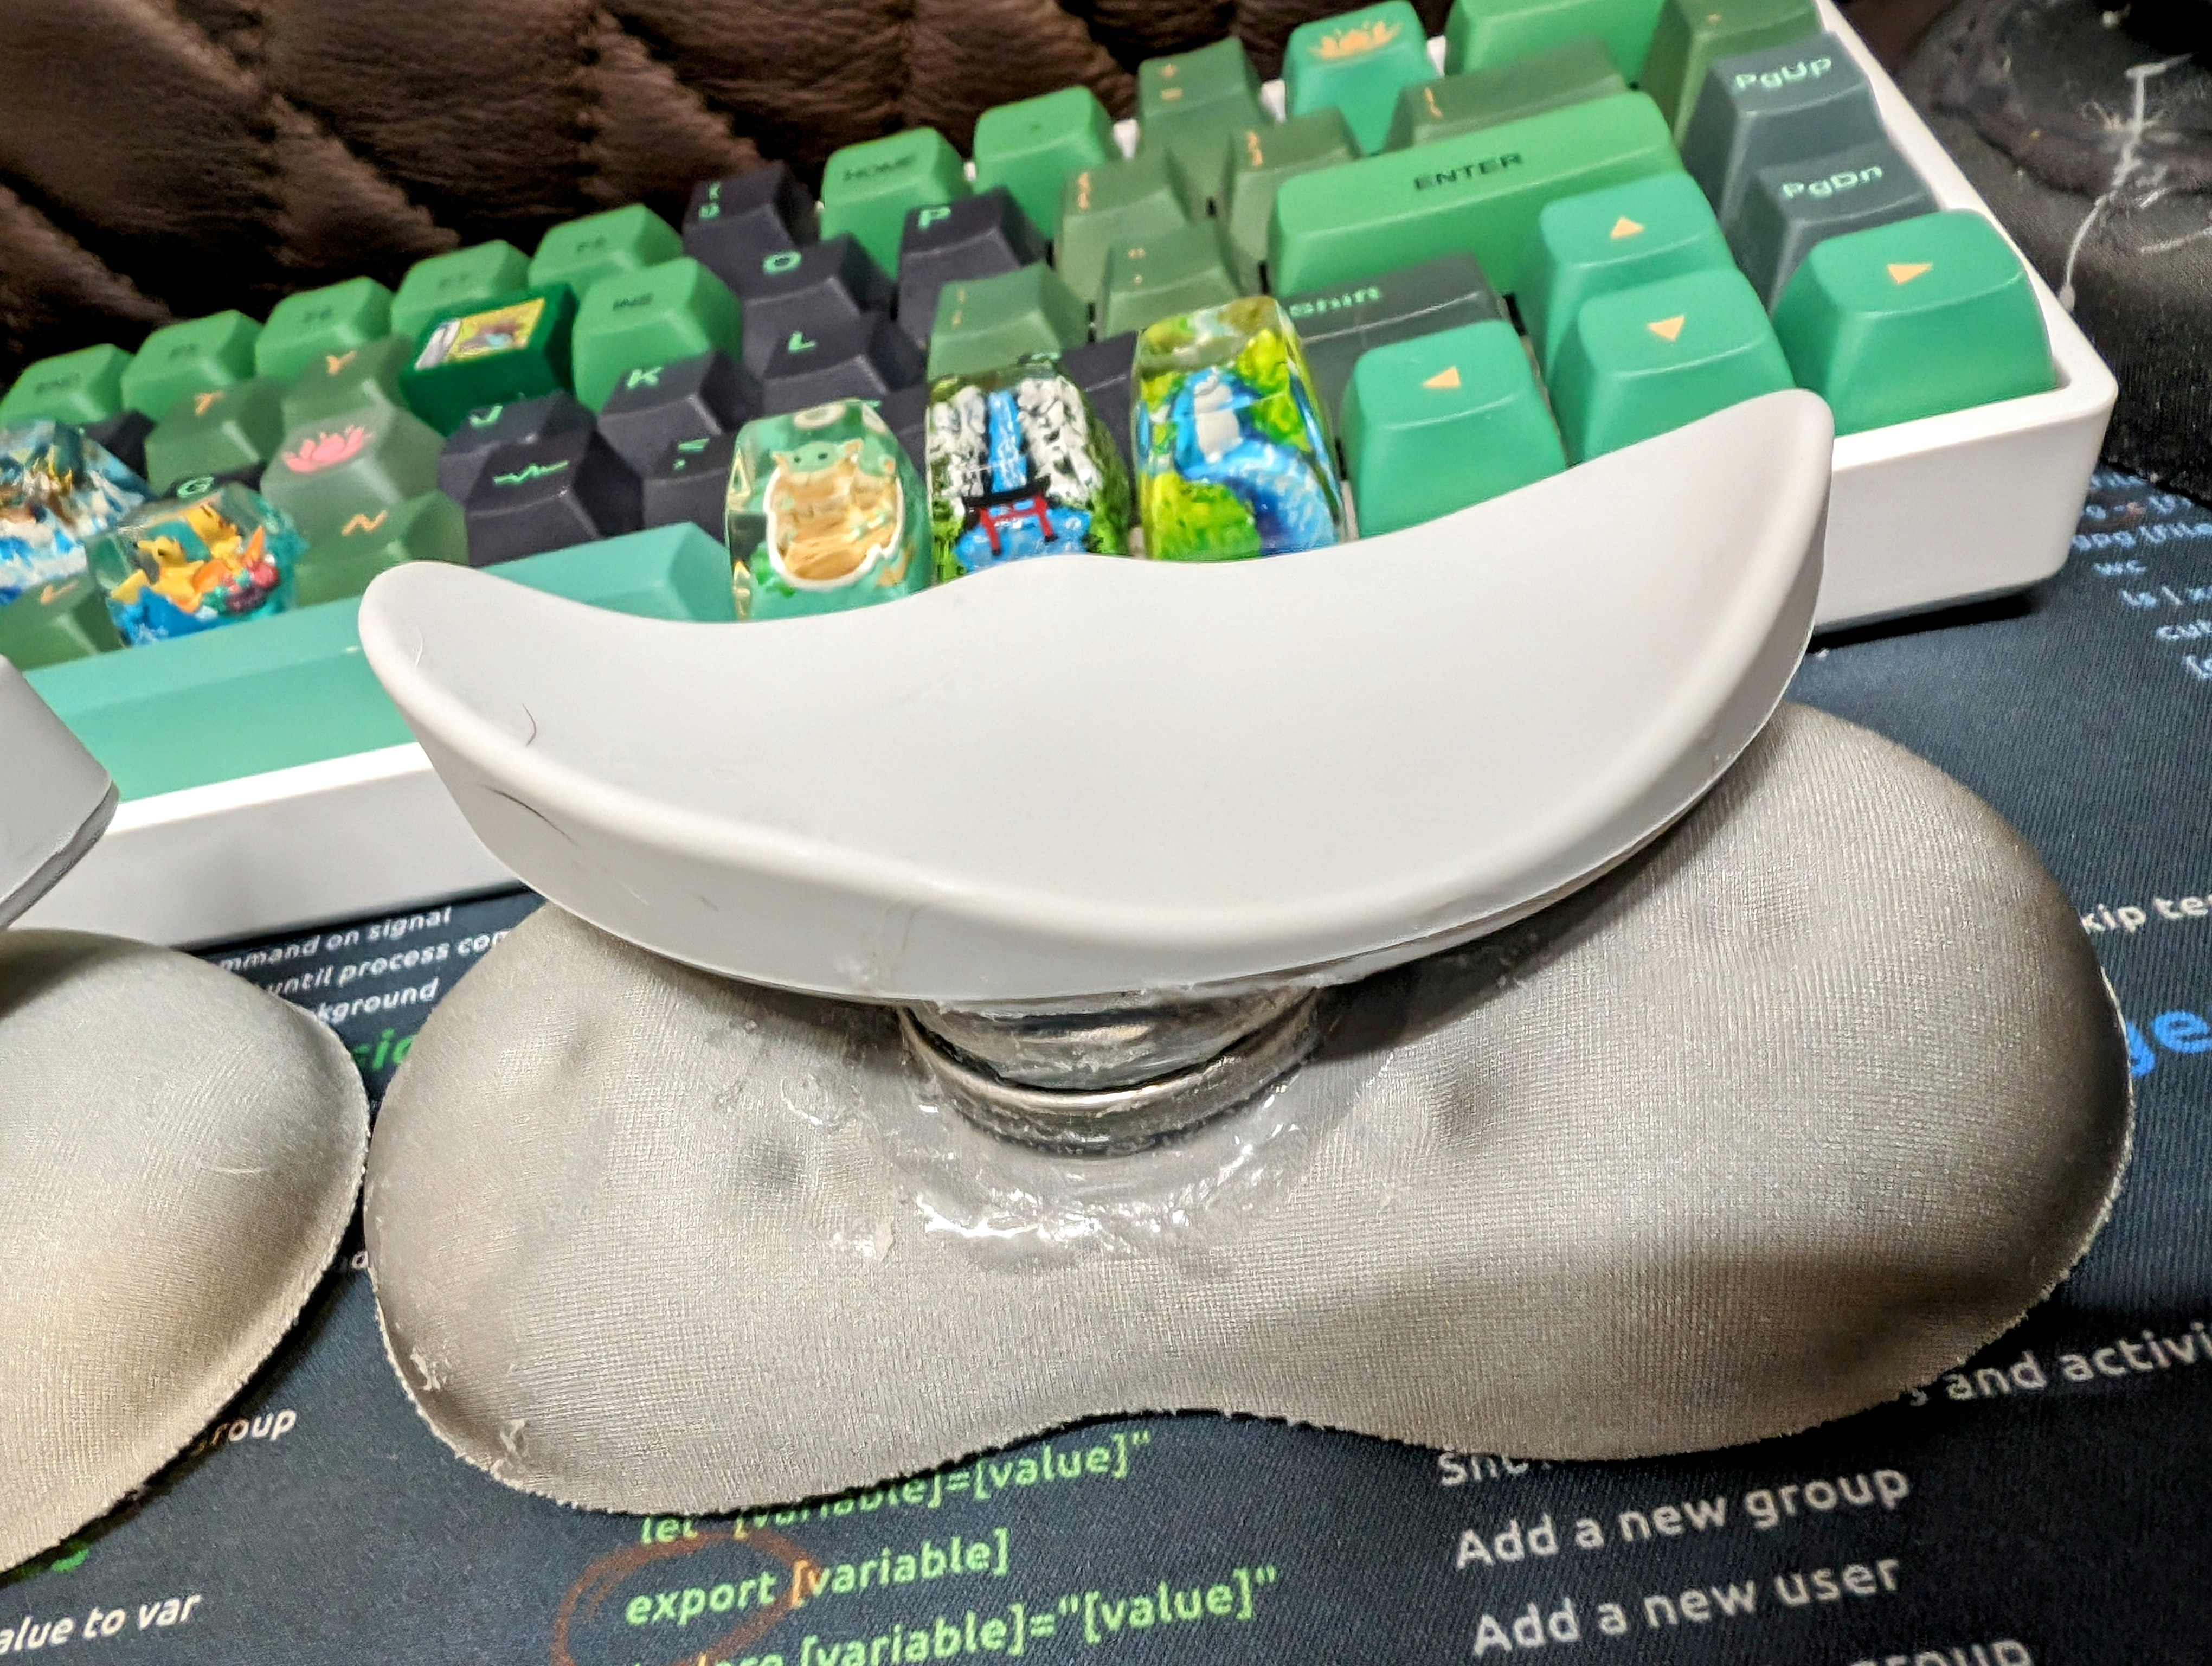
\includegraphics[width=\linewidth]{snorelax.png}
		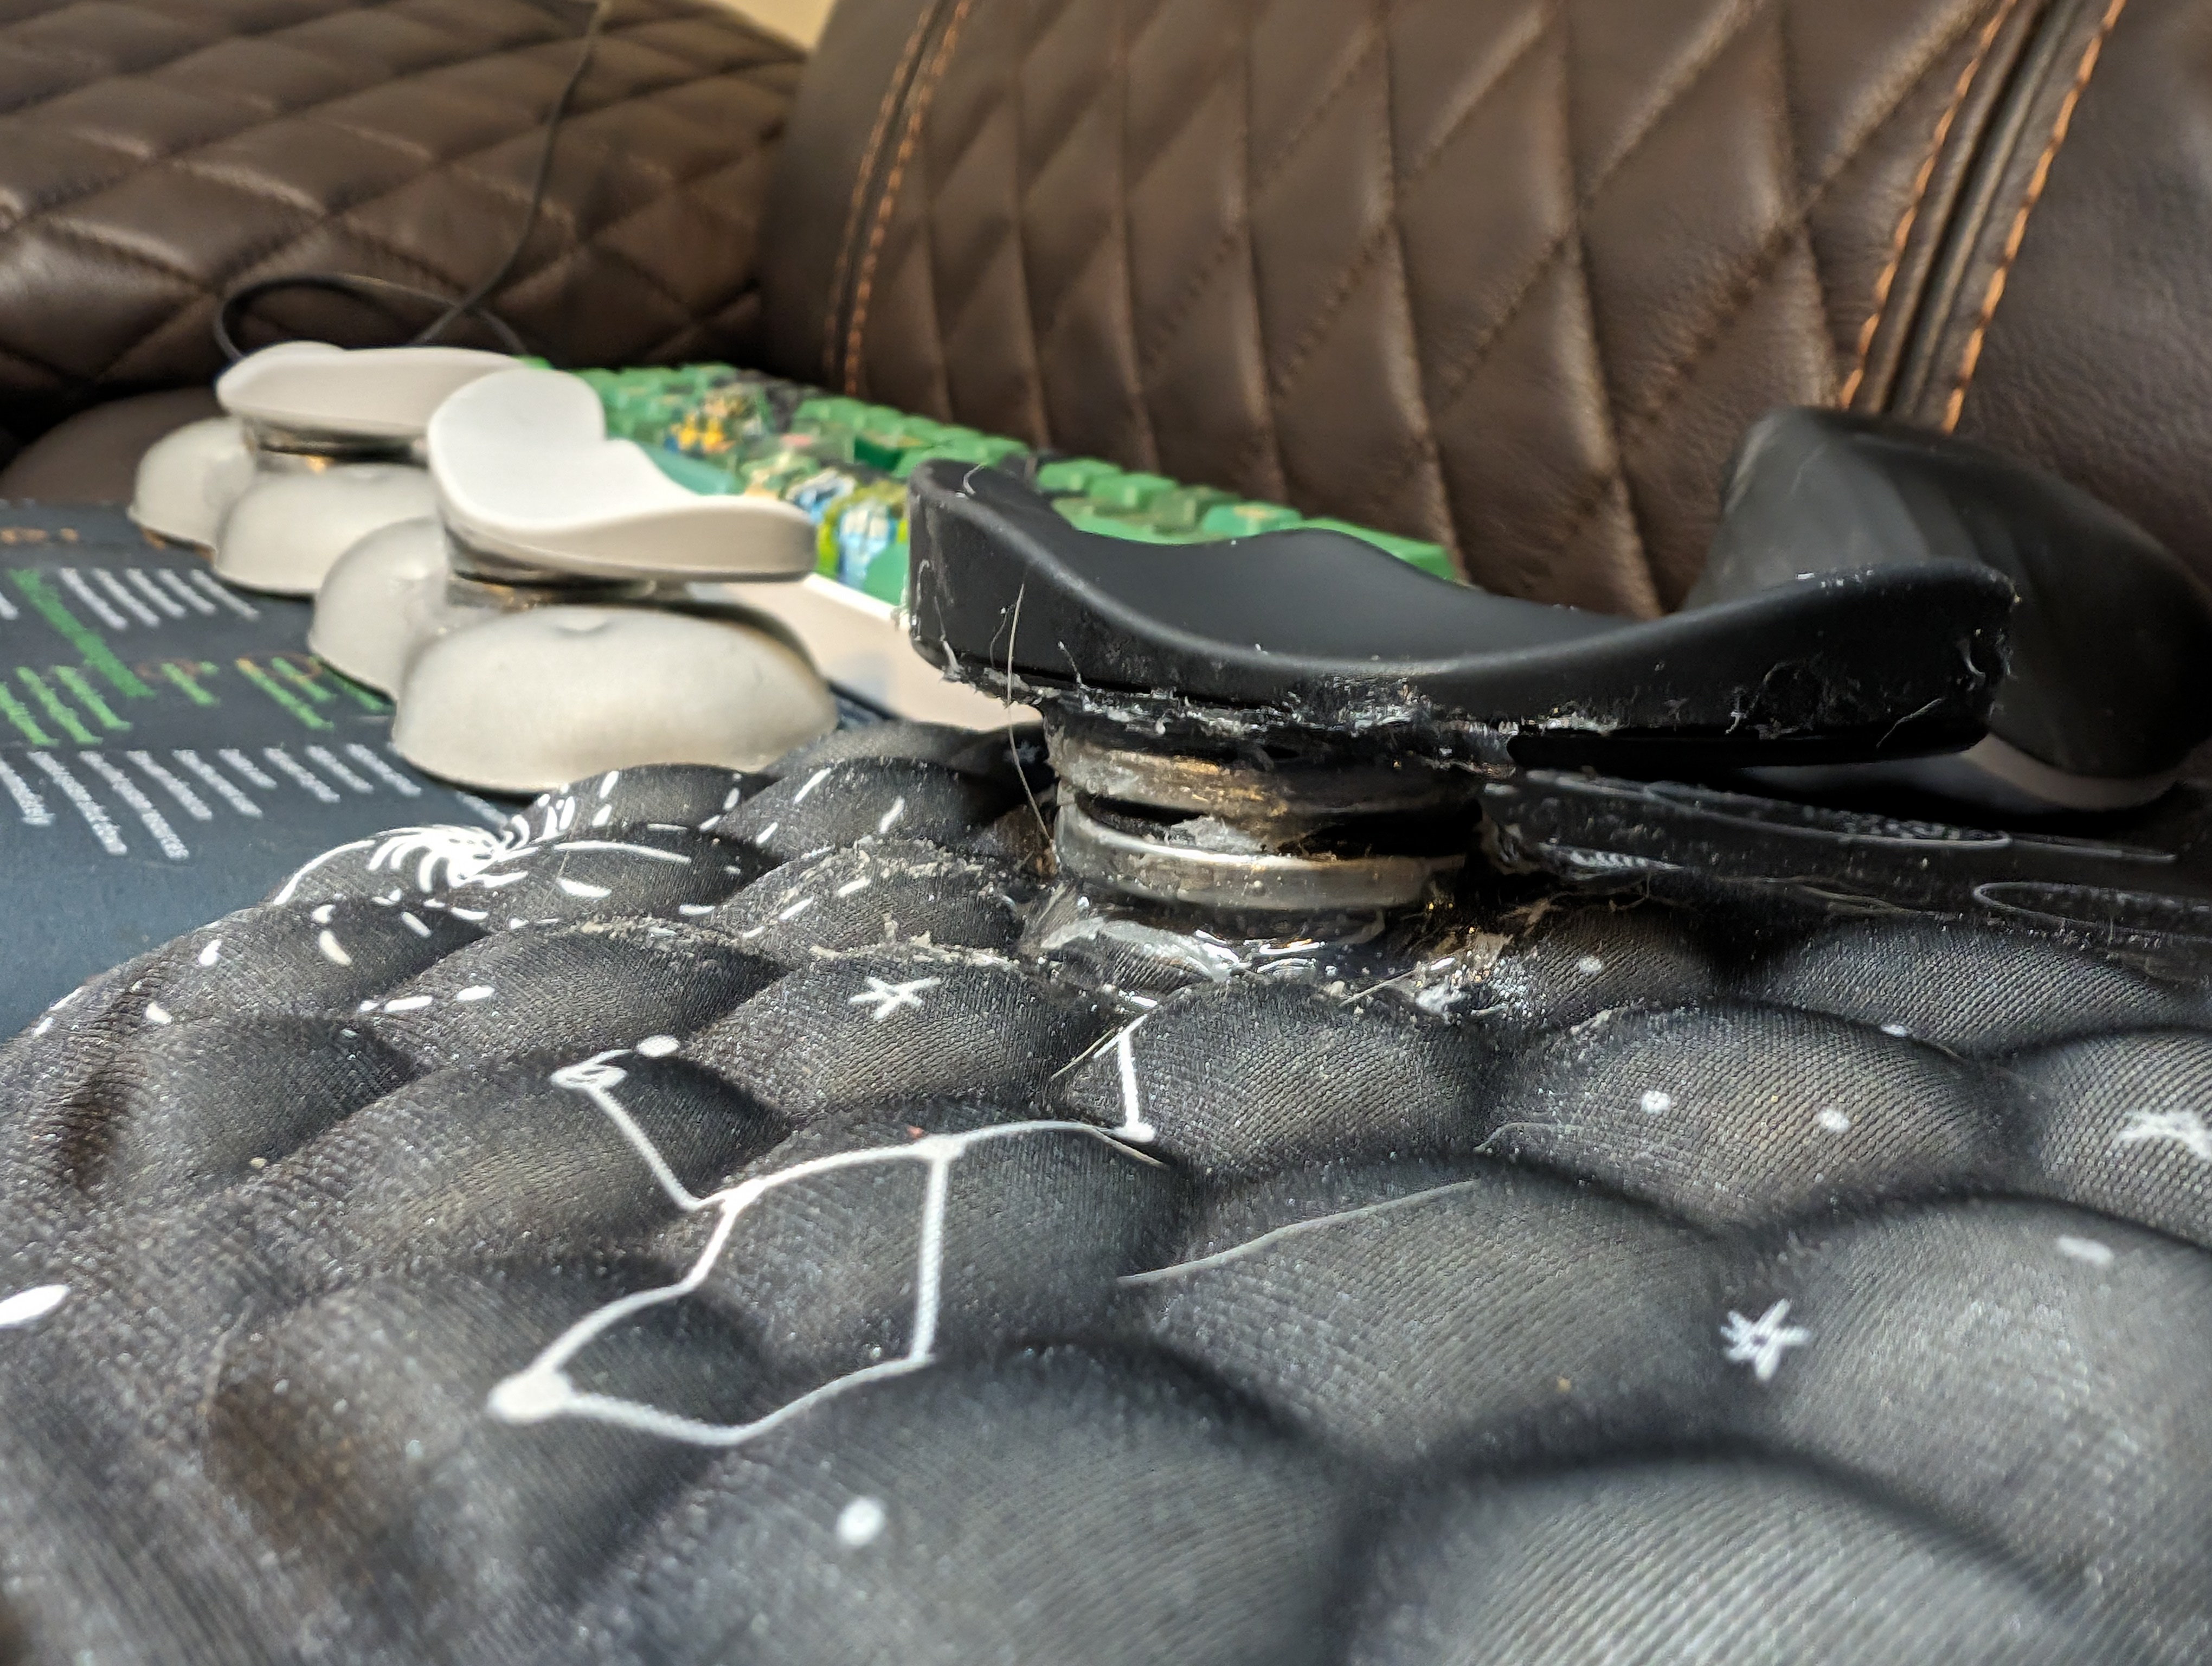
\includegraphics[width=\linewidth]{whole.png}
	}
	
	% footer
	% generate qr code from https://www.qr-code-generator.com/ and replace qr_code.png
	% default: barcode on the left
	\makefooter{images/white-red.png}{images/qr-code.png}
	
	% replace with this like for barcode on the right
	%\makealtfooter{images/uni_logo.png}{images/qr-code.png}
	
\end{document}